\documentclass{article}
\usepackage[T1]{fontenc}
\usepackage{lmodern}
\usepackage{amsmath}
\usepackage{graphicx}
\usepackage{float}
\usepackage{listings}
\usepackage{xcolor}
\usepackage[polish]{babel}

\usepackage[a4paper, margin=2.54cm]{geometry}

\title{Praca domowa 2\\Metoda gradientowa oraz\\
minimalizacja wybranej funkcji}
\author{Damian Jankowski s188597}

\begin{document}

\maketitle

\section{Wstęp}
Tematem pracy domowej jest zapoznanie się z minimalizacją funkcji
metodą gradientową. W tym celu wybrałem funkcję
$f(x, y) = 3x^2-2xy+3y^2-2x-4y$. Poszukiwanie minimum funkcji
zaczęłem od wybrania losowego punktu startowego $X_0$ z zakresu
$-100 \le x \le 100$ oraz $-100 \le y \le 100$.

\begin{figure}[H]
    \centering
    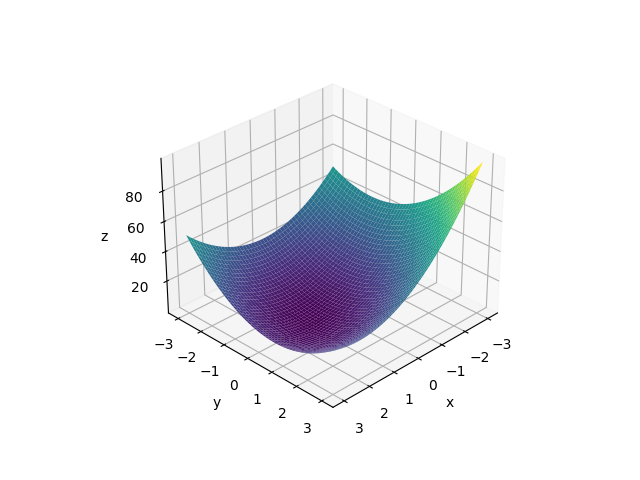
\includegraphics[width=0.5\textwidth]{function.png}
    \caption{Wykres funkcji $f(x, y)$}
\end{figure}


\section{Zadanie}
Do wyznaczenia minimum funkcji metodą gradientową trzeba użyć
wzoru:
\begin{equation}
X_{k+1} = X_k - \alpha_k \nabla f(X_k)
\end{equation}
gdzie $\alpha_k$ jest stałą kroku, 
a $\nabla f(X_k)$ jest gradientem
funkcji $f(x, y)$ w punkcie $X_k$.

Gradient funkcji $f(x, y)$ to inaczej wektor pochodnych
cząstkowych:
\begin{equation}
\nabla f(x, y) = \left( \frac{\partial f}{\partial x}, \frac{\partial f}{\partial y} \right)
\end{equation}
W przypadku wybranej funkcji gradient ma postać:
\begin{equation}
\nabla f(x, y) = {6x-2y-2 \choose -2x+6y-4}
\end{equation}
Dla tego przykładu stała kroku $\alpha_k = 0.1$ natomiast
warunek zakończenia to ilość iteracji $k \ge 25$

\section{Przykładowe obliczenia}

Dla przykładowego punktu startowego $X_0 = (1, 1)$
wyznaczenie 5 kolejnych punktów wygląda następująco:
\begin{equation*}
    \begin{aligned}
X_1 &= {{1} \choose {1}} - 0.1 {{6 - 2 - 2}\choose{-2 + 6 - 4}} = {{0.8} \choose {1}} \\
X_2 &= {{0.8} \choose {1}} - 0.1 {{6 \cdot 0.8 - 2 \cdot 1 - 2}\choose{-2 \cdot 0.8 + 6 \cdot 1 - 4}} = {{0.72} \choose {0.96}} \\
X_3 &= {{0.72} \choose {0.96}} - 0.1 {{6 \cdot 0.72 - 2 \cdot 0.96 - 2}\choose{-2 \cdot 0.72 + 6 \cdot 0.96 - 4}} = {{0.68} \choose {0.928}} \\
X_4 &= {{0.68} \choose {0.928}} - 0.1 {{6 \cdot 0.68 - 2 \cdot 0.928 - 2}\choose{-2 \cdot 0.68 + 6 \cdot 0.928 - 4}} = {{0.656} \choose {0.9072}} \\
X_5 &= {{0.656} \choose {0.9072}} - 0.1 {{6 \cdot 0.656 - 2 \cdot 0.9072 - 2}\choose{-2 \cdot 0.656 + 6 \cdot 0.9072 - 4}} = {{0.644} \choose {0.8944}}
    \end{aligned}
\end{equation*}


\begin{figure}[H]
    \centering
    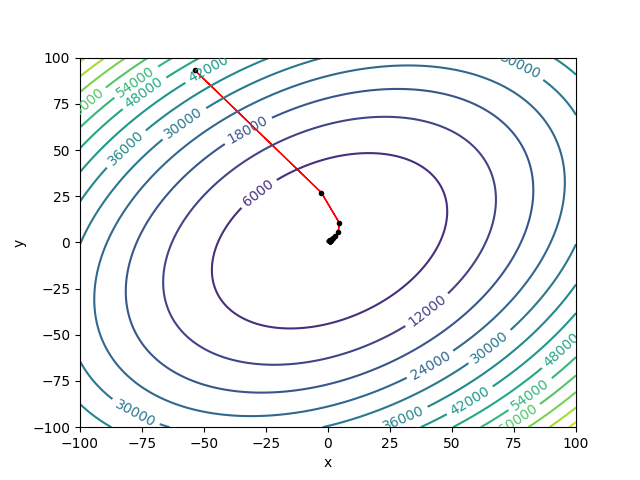
\includegraphics[width=0.5\textwidth]{plot.png}
    \caption{Rzut 2D funkcji $f(x, y)$ oraz kolejne kroki
    minimalizacji metodą gradientową} {dla wylosowanego punktu startowego}
\end{figure}


\section{Kod programu}
\lstinputlisting[
language=python,  
basicstyle=\small\tt,
keywordstyle=\color{blue},
backgroundcolor=\color{cyan!10}
]{main.py}

\end{document}
